\section{Results and Discussion}
\label{sec:results}

Using a fiducial volume containing 34\,kg of liquid xenon and 224.6~live days of data yields 764 events observed  in the region of interest.
This number is compatible with the expectation of $756 \, \pm \, 5 \,{\rm (stat)} \, \pm 55\, {\rm (syst)}$ events from the background only hypothesis. 
Figure~\ref{fig:dataVSbkg} shows the distribution of  events  in the region of interest, where the bottom panel displays the ratio
between data and expected background. The grey and orange shaded areas represent the statistical and systematic uncertainty 
on the background expectation, respectively. The expected signal for a WIMP mass of 100\,GeV/c$^2$, and normalised to a total of 50 events, is also shown.

%\newpage

\begin{figure}[t!]
  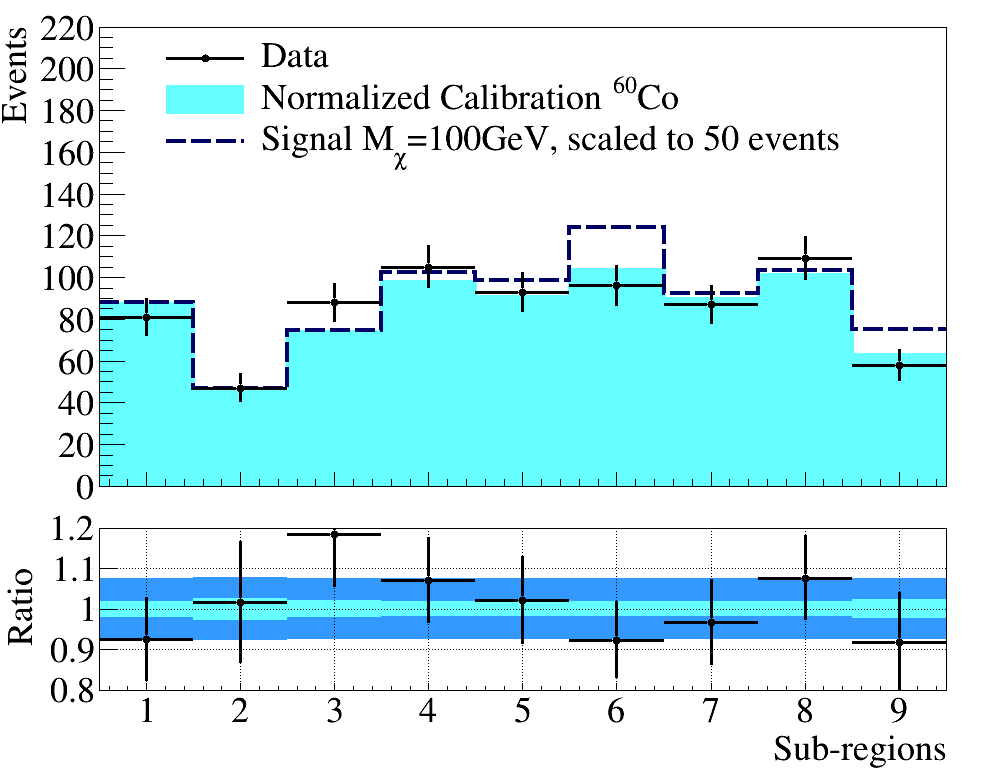
\includegraphics[width=\linewidth]{images/data_vs_bkg.png}
  \caption{Distribution of  observed events  in the region of interest (data points), along with the normalised distribution from calibration data (filled histogram). The bottom panel displays the ratio
between data and expected background, where the grey and orange shaded areas represent the statistical and systematic uncertainty 
on the background expectation, respectively. The expected signal for a WIMP mass of 100\,GeV/c$^2$ (blue dashed), and normalised to a total of 50 events, is also shown.}
  \label{fig:dataVSbkg}
\end{figure}

 

This result is interpreted via a binned profiled likelihood approach by means of the test statistic $\tilde{q}$
and its asymptotic distributions, as  described in \cite{asympt}. 
Assuming  an isothermal WIMP halo with a local density of $\rho_{\chi} \, = \, 0.3$\,GeV/cm$^3$, a local circular velocity of $v_0 \,= \, 220$\,km/s, and a galactic escape velocity of $v_{\rm{esc}} \, = \, 544$\,km/s, 
\textcolor{blue}{other assumptions...,} a 90\% CL$_s$~\cite{cls} confidence level upper limit on the spin-dependent inelastic WIMP-nucleon cross section as a function of WIMP mass is computed. We employ the nuclear structure factors as calculated in \cite{Baudis:2013qla}, based on state-of-the-art large-scale shell-model calculations, with chiral effective field theory WIMP-nucleon currents. 

\begin{figure}[h]
  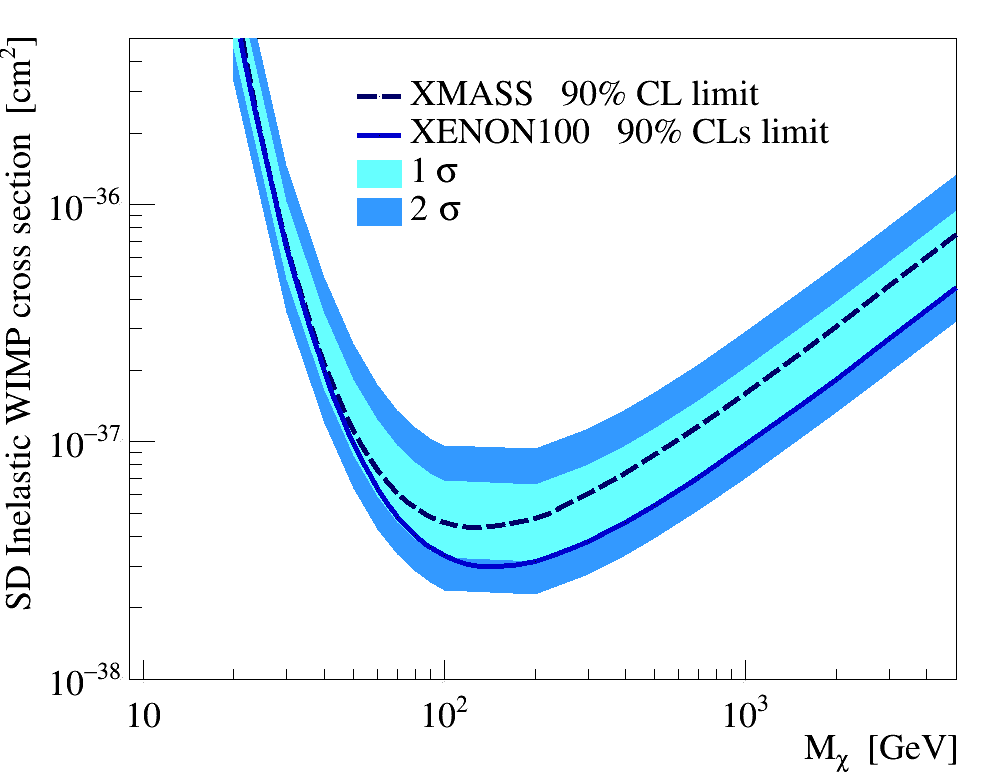
\includegraphics[width=\linewidth]{images/limit_reb.png}
  \caption{Upper limit (black curve) on the spin-dependent, inelastic WIMP-nucleon cross section as a function of WIMP mass.  The expected median sensitivity (dashed curve) along with the relative one (green area) and two (yellow area) standard deviation uncertainty is also shown. This result is compared to the upper limit (at 90\% C.L.) obtained by the XMASS experiment (red curve)~\cite{Uchida:2014cnn}.}
  \label{fig:limits}
\end{figure}


Our result is shown in Figure~\ref{fig:limits}, together with the expected median sensitivity and its relative one and two  standard deviation uncertainty.
The most constraining upper limit is  $3.3 \times 10^{-38}$\,cm$^{2}$ (at 90\% CL$_s$ confidence level) is for a WIMP of mass 100\,GeV/c$^2$. 

This results is compared to the one obtained by the XMASS experiment~\cite{Uchida:2014cnn}, a single phase liquid xenon detector, which used a fiducial volume containing 41\,kg of LXe and 165.9~live days of data. \textcolor{blue}{Decide which other experiment to also plot - DAMA LXe? However only XMASS uses the same form factors as we do.}


Our limit improves upon the XMASS result and constrains new parameter space for the spin-dependent, inelastic scattering cross section. While these upper limits are not competitive to spin-dependent, elastic scattering results, as obtained by XENON100~\cite{Aprile:2013doa} and LUX~\cite{Akerib:2016lao} (with a cross section minimum of $\sim2 \times 10^{-40}$\,cm$^{2}$, at 90\% C.L.,  for a 100\,GeV/cm$^2$ WIMP), our results set the pathway for a sensitive search of inelastic WIMP-nucleus scattering in running or upcoming liquid xenon experiments such as XENON1T~\cite{Aprile:2015uzo}, XENONnT~\cite{Aprile:2015uzo},  LZ~\cite{Akerib:2015cja}, and DARWIN~\cite{Aalbers:2016jon}. In these larger detectors, with lower intrinsic backgrounds from $^{85}$Kr and $^{222}$Rn decays, and improved self-shielding, the electronic recoil background will be reduced by a few orders of magnitude with respect to XENON100, and ultimately dominated by solar neutrino interactions~\cite{Baudis:2013qla}. 

The discovery of this interaction channel would be a clear signature for a spin-dependent nature of the interaction, and would provide a potential handle  to constrain the WIMP mass~\cite{Baudis:2013bba}.

%\newpage
